\section{Experiments and Results}
\label{sec:experiments}

\begin{figure*}[t!]
    \centering
    \subfloat[]{
            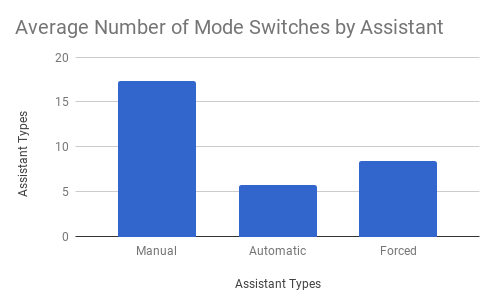
\includegraphics[width=0.25\textwidth]{figs/mode_full}
            \label{fig:mode_full}
        }
        \subfloat[]{
            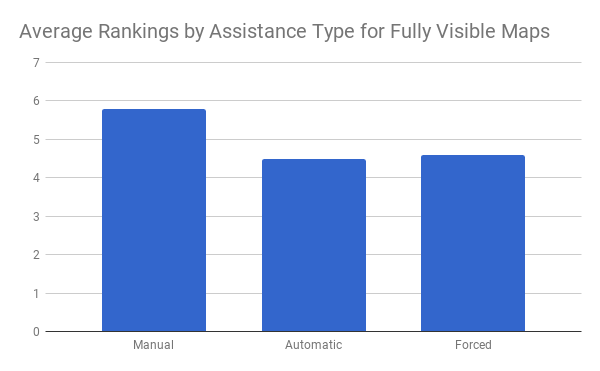
\includegraphics[width=0.25\textwidth]{figs/rankings_full} 
            \label{fig:rankings_full}
        }
        \subfloat[] {
            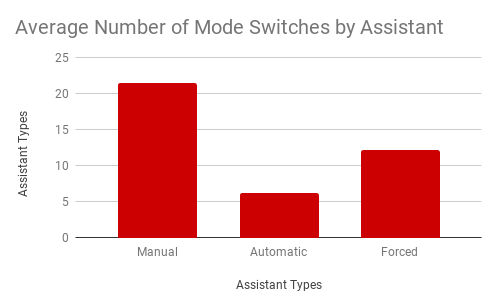
\includegraphics[width=0.25\textwidth]{figs/mode_partial}
            \label{fig:mode_partial}
        }
        \subfloat[] {
            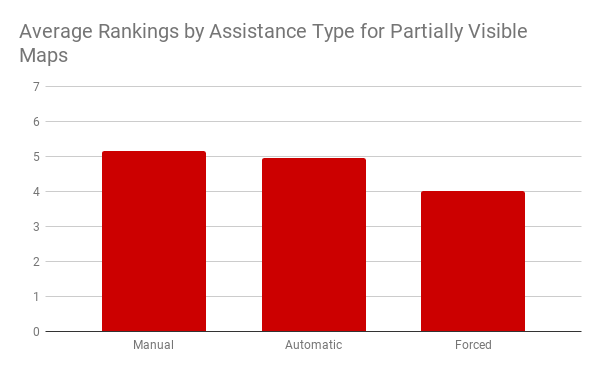
\includegraphics[width=0.25\textwidth]{figs/rankings_partial}
            \label{fig:rankings_partial}
        }
        \label{fig:charts}
         \caption{\protect\subref{fig:mode_full}~The average number of mode switches made the user in the fully-visible map for each assistance type. \protect\subref{fig:rankings_full}~The average rankings for how much the user trusted the robot for each assistance type in the fully-visible map. \protect\subref{fig:mode_partial}~The average number of mode switches made the user in the partially-visible map for each assistance type, \protect\subref{fig:rankings_partial}~The average rankings for how much the user trusted the robot for each assistance type in the partially-visible map. }
\end{figure*}

To assess trust, we primarily considered the number of mode switches made by the user, and secondarily considered the comfort rankings submitted by the user; we concluded that the number of mode switches would be an accurate measure for trust because this would show if the user had trusted the robot enough that there were significantly fewer mode switches, whereas user rankings was used as a secondary metric because comfort doesn’t necessarily equate to trust, and also user rankings are subjective and very dependent on the order of the trials. We chose to perform one-tail t-tests to determine significance in our data, because our hypotheses look specifically for either a significant increase or a significant decrease in the metric, rather than any significant difference. We compare our p-values against $\alpha = 0.05$.

For \hyp{hyp:h1}, we did not expect the user to be satisfied with the forced assistance type because if they could see the entire map, we believed they would be less likely to trust the robot's assistance. Performing a one-tail t-test to compare the number of mode switches, we saw a $p = 1.88 \times 10^{10}$, which is very significant. This shows that the users manually switched modes significantly less on the automatic assistance type trials in comparison with the manual assistance type trials~(\figref{fig:mode_full}).  

In contrast, while looking at the survey data for fully-visible environment~(\figref{fig:rankings_full}), the lesser rankings for forced/automatic versus manual is significant $p =  0.009$ and $p = 0.003$ respectively). This demonstrates that, while the users may have trusted the robot more, in terms of mode-switching, they were not comfortable with the assistance. As we are prioritizing the mode switching as our metric for trust, we do not reject the first hypothesis, but we note that the trust was prevelant but the comfort was not. Additionally, we accept that our hypothesis was wrongly limited, given that the number of mode switches for forced assistance types was also highly significant, with a $p = 2.29 * 10^5$. To conclude, for \hyp{hyp:h1}, users trusted the robot's automatic and forced assistance but were not comfortable with it.

For \hyp{hyp:h2} we expected that, because the user had a limited understanding of the environment in comparison with the robot, the user would be more inclined to trust the robot's assistance. There obvious decrease in the number of mode switched for both forced and automatic versus manual~(\figref{fig:mode_partial}). Because the $p = 0.01$ for forced versus manual and $p = 4.58 * 10^{-10}$ for automatic versus forced, we conclude that both results are significant. Additionally, users’ trust rankings for each assistance type are very similar; $p=0.03$ for forced and $p=0.35$ for automatic~(\figref{fig:rankings_partial}). Therefore, users do not mind the assistance given by the automatic in partially-visible environments but are still not comfortable with forced. To conclude, for \hyp{hyp:h2}, we accept it for both the forced and automatic assistance types.

Lastly, for \hyp{hyp:h3} we hypothesized that there would be a decrease in time taken to reach the goal when the users are given forced/automatic assistance rather than manual control. \footnote{Note that this hypothesis is regardless of map type; however, we expect that the full and partial maps would have differing times by design and so we still compare this data separately.} 
For each map type, the assistance types demonstrate very similar times~(\figref{fig:time_full}, \figref{fig:time_partial}). All the p-values are greater than $\alpha = 0.05$~(\figref{fig:time_p_values}), and so we have no significant differences in time. Thus, we reject \hyp{hyp:h3}. Intuitively, we believe that while mode switching may have been significantly decreased, users still required time to reassess their situation after the robot switched modes, and so the times balanced out regardless of the robot’s assistance.

